\chapter{Bleach} \label{cap:metodologia}

\begin{displayquote}
    \begin{center}
        \textit{``Bullet, Claw, Battle Flag, Short Sword. With my fingers bent, I wait for you.''}
    \end{center}
\end{displayquote}

\begin{flushright}
   \textit{-- NORIAKI KUBO}
\end{flushright}

\section{Introduction}
This chapter is dedicated to provide a detailed explanation about the Bleach programming language. Firstly, a brief overview of Bleach's features is presented by showcasing a few programs written in the language. Then, a detailed breakdown of each of its components and features is shown. Afterwards, the challenges encountered during the development of this project are presented, as well as decisions and trade-offs made. Finally, a comparison between Bleach and the previous languages introduced is presented, as well as a discussion about how Bleach can be properly used to its fullest in undergraduate Compilers courses.

\section{Bleach Overview}
As previously mentioned, this section is dedicated to showcase a few of Bleach's features through the exposition of simple, yet useful, programs to the reader. It is expected that the reader has some familiarity programming in other languages, such as C \cite{kernighan1988c}, C++ \cite{strousrup2000c++}, JavaScript \cite{javascript_language}, Lox \cite{nystrom2021crafting}, Python \cite{python_language} or Ruby \cite{ruby_language}, so the similarities between Bleach and these languages make themselves more evident.

\newpage

The first example of Bleach program shown below is the simplest and most famous one known in Computer Science: The "Hello, World!" program: \newline
\begin{lstlisting}
print "Hello, World!"; // "Hello, World!"
\end{lstlisting}


Next, there is a Bleach program that shows the combined usage of recursive functions, if-else statements and arithmetic operators to calculate the factorial of a number: \newline
\begin{lstlisting}
function factorial(n){
  if(n == 0){
    return 1;
  }else{
    return n * factorial(n - 1);
  }
}

print factorial(5); // 120
\end{lstlisting}


After this, a Bleach program that illustrates the usage of for loops and the native \texttt{list} type in order to build a list that contains some information about numbers from 0 to 10: \newline
\begin{lstlisting}
function main(){
  let numbersInfo = [];
  for(let i = 0; i <= 10; i = i + 1){
    if(i % 2 == 0){
      numbersInfo.append(i + " is even!");
    }else{
      numbersInfo.append(i + " is odd!");
    }
  }
  print numbersInfo;
}

main();
\end{lstlisting}

\newpage


Now, there is a Bleach program that implements a function which receives the coefficients of a quadratic equation in order to compute its roots: \newline
\begin{lstlisting}
function quadraticEquationSolver(a, b, c){
  let delta = std::math::pow(b, 2) - 4 * a * c;
  let x1 = (-b + std::math::sqrt(delta))/(2 * a);
  let x2 = (-b - std::math::sqrt(delta))/(2 * a);

  return [x1, x2];
}

print quadraticEquationSolver(1, 0, -4); // [2, -2]
\end{lstlisting}


Below, there is a Bleach program that illustrates Object-Oriented features of the language, such as: classes, instances, attributes, methods, overriding and inheritance: \newline
\begin{lstlisting}
class Shape{ // Base Class
  method init(name){
    self.name = name;
  }

  method str() {
    return "This is a " + self.name + ".";
  }

  method area(){ // To be overridden by subclasses
    return 0;
  }
}

class Circle inherits Shape{ // Derived Class
  method init(radius){
    super.init("Circle"); // Call the Base Class constructor
    self.radius = radius;
  }

  method area(){
    return std::math::pow(self.radius, 2) * 3.14159;
  }
}

class Triangle inherits Shape{ // Derived Class
  method init(base, height) {
    super.init("Triangle"); // Call the Base Class constructor
    self.base = base;
    self.height = height;
  }

  method area(){
    return (self.base * self.height) / 2;
  }
}

let c = Circle(5);
let t = Triangle(3, 7);

// This is a Circle. It has an area of 78.539749999999998 units.
print c + " It has an area of " + c.area() + " units.";
// This is a Triangle. It has an area of 10.5 units.
print t + " It has an area of " + t.area() + " units.";
\end{lstlisting}

And finally, a Bleach program that shows its capability with dealing with user-input and writing to \texttt{.txt} files: \newline
\begin{lstlisting}
function writeToFile(){
  let userInput = std::io::readLine();
  std::io::fileWrite("output.txt", "w", userInput, true);

  userInput = std::io::readLine();
  std::io::fileWrite("output.txt", "a", userInput, false);

  return;
}

writeToFile();
\end{lstlisting}


\section{Bleach Features}
\subsection{Introduction}
Bleach is a high-level and dynamically-typed programming language designed with the intent to be used as a teaching tool in undergraduate Compilers courses. The motivation behind its creation lies in the fact that according to the studies mentioned in section 3 and in my personal experience, a more incremental and practice-oriented approach when teaching such courses is more rewarding to the teaching staff and to the students, especially when it comes to grasp the core concepts of it. Last but not least, as it is shown in this chapter and in the next one, Bleach is a more complete language when compared to Cool and MiniJava, which might better capture students' interest in implementing a programming language that resembles those they are used to utilizing in their daily lives.

\subsection{Data Types}
Bleach has 5 built-in data types made available to the user. Such types are divided into scalar types  and compound types.

Scalar types are types that can represent a single value. In Bleach, there are 3 scalar data types: \texttt{bool}, \texttt{nil} and \texttt{num}.
\begin{itemize}
    \item \texttt{bool}: This data type is used to represent one of two possible values: \texttt{true} or \texttt{false}. Such values are used to express logical conditions and to control the execution of certain parts of a program's source code.
    
    In this context, it is important to mention that Bleach takes inspiration from Ruby and other modern programming languages and implements the concept of "truthy" and "falsey" values in order to evaluate the truthiness or the falseness of values when they are being evaluated inside \texttt{if} statements, loops (\texttt{while}, \texttt{do-while}, \texttt{for}) and ternary operators (\texttt{condition ? expression\_1 : expression\_2}).

    Essentially, this means that, in Bleach, values of any type (built-in or user-defined) can be used in places where a value of type \texttt{bool} is expected. Moreover, Bleach opted to follow the same convention of Ruby in this matter, which says:

    \begin{itemize}
        \item \textbf{"Falsey" values:} \texttt{false}, \texttt{nil}.
        \item \textbf{"Truthy" values:} Any other value that is not \texttt{false} nor \texttt{nil}.
    \end{itemize}
    
    \item \texttt{nil}: This one is an old acquaintance for most programmers. The \texttt{nil} type has just one possible value, the \texttt{nil} value. In short this value conveys the idea of "no value" or the "absence of a value".

    In other programming languages, this concept appears in other forms, like: \texttt{NULL}, \texttt{nullptr}, \texttt{null}, \texttt{None}, \texttt{nil}, and others. Since Bleach has some influence from Ruby, it adopted \texttt{nil}.
    
    \item \texttt{num}: In favor of simplicity, Bleach has only one type to represent numbers: the \texttt{num} type. This type can be used to represent both integers and floating-point numbers.

    Behind the scenes, the \texttt{num} type is implemented with a double-precision floating-point type, which allows Bleach to cover a lot of territory when it comes to numerical values while still keeping the simplicity initially envisioned for the language.
    
    Finally, with respect to numerical literals, Bleach has support for only basic integer and decimal literals, such as: \texttt{23}, \texttt{42}, \texttt{3.14159}, \texttt{2.71828}, \texttt{-10.4}.
    
\end{itemize}

Compound types are types that can group multiple values into one. In Bleach, there are 2 compound types: \texttt{list} and \texttt{str}.
\begin{itemize}
    \item \texttt{list}: Taking inspiration from Python \cite{python_language}, Bleach has this type. Here, the \texttt{list} type represents a linear-sequence of elements. As previously stated, Bleach is a dynamically-typed language, just like Python. Thus, the \texttt{list} type can store values of different types with no issues. Moreover, Bleach has support for \texttt{list} literals, just as the ones shown below:\newline

    \begin{figure}[H]
        \centering
        \begin{lstlisting}
let l0 = [0, 1, 2, 3, 2.71, 3.14159];
let l1 = ["hello", "there"];
let l2 = [];
let l3 = [false, "Brazil", 9.98, nil];
        \end{lstlisting}
        \caption{Examples of \texttt{list} literals in Bleach.}
    \end{figure}

    Finally, as in Python, the \texttt{list} type in Bleach has the following useful methods that makes the student's life easier when working with this type.
    
    \begin{itemize}
        \item \texttt{append}: Responsible for adding one value of any type to the end of the \texttt{list} value it was called on. Returns \texttt{nil}.
        \item \texttt{clear}: Method responsible for deleting every element that is currently stored inside the \texttt{list} value it was called on. Returns \texttt{nil}.
        \item \texttt{empty}: Responsible for checking whether the \texttt{list} value it was called on currently has values stored inside it or not. Returns a \texttt{bool} value.
        \item \texttt{fill}: Responsible for resizing the \texttt{list} value it was called on to a provided size and also filling all of its indexes with a provided value of any type. Returns \texttt{nil}; 
        \item \texttt{getAt}: Responsible for returning the value present at the provided index. Returns a value of any type.
        \item \texttt{pop}: Responsible for deleting and returning the last element present inside a \texttt{list} value, if any. Returns a value of any type.
        \item \texttt{setAt}: Responsible for setting the value stored at the provided index to the value that was provided. Returns \texttt{nil}.
        \item \texttt{size}: Responsible for checking and returning the current amount of elements that the \texttt{list} value it was on called on currently has. Returns a \texttt{num} value.
    \end{itemize}

    Last but not least, it is important to highlight that any misuse of the methods presented above will result in a runtime error during the program's execution.

    \item \texttt{str}: Also taking inspiration from Python \cite{python_language}, Bleach has this type. The \texttt{str} type represents an indexed-sequence of characters (a string), typically used to store and manipulate text. Just as the \texttt{list} type, Bleach also has support for literal values of this type:

    \begin{figure}[H]
        \centering
        \begin{lstlisting}
let s0 = "Ichigo Kurosaki";
let s1 = "Grimmjow Jaegerjaquez";
let s2 = "Bazzard Black";
let s3 = "Jugram Haschwalth";
        \end{lstlisting}
        \caption{Examples of \texttt{str} literals in Bleach.}
    \end{figure}

    There are other aspects about the \texttt{str} type that must be mentioned.

    First of all, it is important to recall that it is a sequence type. In short, it means that values of this type can be indexed. In a string, indexing usually allows the programmer to access individual characters from the value, which, in the Bleach programming language, are also values of \texttt{str} type.

    Also, as seen in Figure 4.8, in Bleach, literals values of this type are always enclosed by double quotes (\texttt{""}).

    Finally, as in Python, this type has the following useful methods available:

    \begin{itemize}
        \item \texttt{empty}: Responsible for checking whether the \texttt{str} value it was called is equal to \texttt{""} or not. Returns a \texttt{bool} value.
        \item \texttt{find}: Responsible for trying to figure out if the provided sub-string (a \texttt{str} value) exists within the \texttt{str} value the method was called on. Returns a \texttt{num} value which denotes the index at which the sub-string appears, otherwise returns \texttt{-1}. 
        \item \texttt{getAt}: Responsible for returning the \texttt{str} value of length 1 present at the provided index. Returns a \texttt{str} value.
        \item \texttt{length}: Responsible for checking and returning the current amount of characters (which are also values of type \texttt{str}) that the \texttt{str} value it was on called on currently has. Returns a \texttt{num} value.
        \item \texttt{split}: Responsible for generating a \texttt{list} where each value is of \texttt{str} type. This method receives as its unique argument a value of \texttt{str} type that works as the separator. Returns a \texttt{list} value.
        \item \texttt{setAt}: Responsible for setting the value stored at the provided index to the value that was provided (which must be a \texttt{str} value of length \texttt{1}). Returns \texttt{nil}.
        \item \texttt{substr}: Responsible for retrieving a sub-string from the \texttt{str} value it was called on. The method receives two arguments of \texttt{num} type that work as the start and end delimiters. Returns a \texttt{str} value.
    \end{itemize}

\end{itemize}

\subsection{Comments}
Even though it is recommendable that a programmer writes code in a way that is readable and understandable, there are certain scenarios where extra explanation about what certain parts of a program's source code is actually doing is welcomed.

In these specific cases, programmers usually leave comments in their code that the compiler/interpreter will ignore but people reading such code may find helpful.

Given this, Bleach takes inspiration from C \cite{kernighan1988c} when it comes to support for single-line comments and multi-line comments.

\begin{itemize}
    \item \textbf{Single-Line Comments:} In Bleach, a single-line comment starts with two slashes (\texttt{//}), and the comment continues until the end of the line.
    \item \textbf{Multi-Line Comments:} Bleach also has support for multi-line comments. A multi-line comment has a beginning and an ending. The former is denoted by a (\texttt{/*}), while the later is denoted by a (\texttt{*/}). Everything written in-between is considered a comment and, thus, is ignored by the interpreter at runtime.
\end{itemize}

    \begin{figure}[H]
        \centering
        \begin{lstlisting}
// This is a single-line comment.

/*
This  is
a multi-line
comment.
*/
        \end{lstlisting}
        \caption{Examples of \texttt{str} literals in Bleach.}
    \end{figure}

\subsection{Variables}
A variable, as in most programming languages, can be viewed as just a name associated with a storage location in memory. Such storage location is responsible for holding data that can be changed during the execution of a program.

In Bleach this is not different. Variables still have this main functionality. However, they have some particularities that might differ from variables in other programming languages. Such peculiarities are listed below:
\begin{itemize}
    \item In Bleach, all variables are mutable. In other words, once a variable is declared, any amount of assignments are allowed to be performed on this declared variable.
    
    \item A direct consequence of the particularity explained above is that there is no concept of constants in Bleach.
    
    \item In Bleach, to declare a new variable, the \texttt{let} keyword must be used:
    \begin{figure}[H]
        \centering
        \begin{lstlisting}
let s = "A value of type 'str'";
        \end{lstlisting}
        \caption{Example of variable declaration in Bleach.}
    \end{figure}
    
    \item In Bleach, if the declaration of a variable does not have an initializer, then, by default, the variable will store the nil value:
    \begin{figure}[H]
        \centering
        \begin{lstlisting}
let someVariable;
print someVariable; // nil
        \end{lstlisting}
        \caption{Example of variable declaration without an initializer in Bleach.}
    \end{figure}

    \item Since Bleach is a dynamically-typed programming language, variables do not have types associated with them. Instead, it is the value stored inside of a variable that has a type. The most important consequence of this fact is that a variable can hold values of different types at different points in time:
    \begin{figure}[H]
        \centering
        \begin{lstlisting}
let a = "hello";
print a; // "hello"

a = nil;
print a; // nil

a = 3.14 + 2.71;
print a // 5.85
        \end{lstlisting}
        \caption{Example demonstrating the fact that, in Bleach, variables do not have types associated.}
    \end{figure}
\end{itemize}

Bleach also has support for global variables, those that have been declared outside of all functions, methods or classes, making them accessible from any part of the program's source code. One point that makes Bleach kind of unique is the fact that the programmer is allowed to re-declare a global variable anytime:
\begin{figure}[H]
    \centering
    \begin{lstlisting}
let pi = 3.14159;
// Write some code in the global scope.
let pi = 9.51413;
    \end{lstlisting}
    \caption{Example demonstrating re-declaration of global variables in Bleach.}
\end{figure}

As expected from most programming language, Bleach supports local variables, which are those declared within a specific block of code, such as a function, method, an \texttt{if-elif-else} statement or a loop statement (\texttt{while}, \texttt{do-while}, \texttt{for}). In this regard, it's important to remember the reader that the scope of a local variable is limited to the block in which it is defined, meaning it can only be accessed and used within that block. Furthermore, once the block of code finishes executing, the local variable is normally destroyed, and its memory is released.
\begin{figure}[H]
    \centering
    \begin{lstlisting}
function foo(){
  let bar = "This is a local variable";
  print bar; // "This is a local variable"

  return;
}

foo();
    \end{lstlisting}
    \caption{Example demonstrating the usage of local variables in Bleach.}
\end{figure}

As previously shown, variables are declared with the usage of the \texttt{let} keyword. Besides, after declaring a variable, the user is allowed to assign different values of different types at different points in time to the declared variable. To do that, the assignment operator (\texttt{=}) comes into play. However, before showing examples of code snippets that make use of this operator, it's very important to mention two semantic details of assignment in Bleach:
\begin{itemize}
    \item In Bleach, an assignment is an expression, not a statement. This means that every assignment produces a value.
    \begin{figure}[H]
        \centering
        \begin{lstlisting}
let foo;
print foo = 20; // 20
        \end{lstlisting}
        \caption{Example showing the behavior of an assignment expression.}
    \end{figure}
    
    \item Bleach allows the user to assign a value to more than one variable in an assignment expression.
    \begin{figure}[H]
        \centering
        \begin{lstlisting}
let x = 20;
let y = 42;

x = y = 13;

print x; // 13;
print y; // 13;
        \end{lstlisting}
        \caption{Example showing the possibility of assigning a value to multiple variable in a single assignment expression.}
    \end{figure}
\end{itemize}

Lastly, Bleach has support for variable shadowing. In practice, this means that when a variable is declared in an inner scope with the same name of another variable, which was declared in an outer scope, the inner variable "shadows" or hides the variable declared in the outer scope. This means that, until this inner scope ends, every variable reference will "hit" the inner one, not the outer one. In this matter, it is important that in order to create a new scope, the user just needs to use curly braces (\texttt{\{\}}). The two examples presented below show how variable shadowing works in practice in Bleach:
\begin{figure}[H]
    \centering
    \begin{lstlisting}
let a = 42;
print a; // 42

{
  let a = "Hello, there!";
  print a; // "Hello, there!" --> Variable Shadowing in action.
}
print a; // 42
    \end{lstlisting}
    \caption{First example of variable shadowing in Bleach.}
\end{figure}

\begin{figure}[H]
    \centering
    \begin{lstlisting}
let foo = "hi";
print foo; // "hi"

function f(){
  let foo = 42;
  print foo; // 42;

  return;
}
f();

print foo; // "hi"
    \end{lstlisting}
    \caption{Second example of variable shadowing in Bleach.}
\end{figure}


\subsection{Operators}
Operators in a programming language are tools responsible for executing an operation on one or more operands in order to produce a result.

Operators are fundamental building blocks in every programming language, since they allow data manipulation, computations execution, values comparison, and much more.

This subsection is dedicated to introduce the operators Bleach grants to its users and how each of such operators behave. In the end, an operator precedence table will be shown.

\begin{itemize}
    \item \textbf{Unary Operators:} These operators expects just one operand. Bleach has 2 operators that fall in this class.
        \begin{itemize}
            \item \textbf{Arithmetical:}
                \begin{itemize}
                    \item \textbf{Negation} (\texttt{-}): Negates the value of an operand of type \texttt{num}.
                    \begin{figure}[H]
                        \centering
                        \begin{lstlisting}
let n = 42;
print -n; // -42
                        \end{lstlisting}
                        \caption{Example of usage of the "negation" operator (\texttt{-}).}
                    \end{figure}
                \end{itemize}
            \item \textbf{Logical:}
                \begin{itemize}
                    \item \textbf{Not} (\texttt{!}): Inverts the value of an operand of type \texttt{bool}.
                    \begin{figure}[H]
                        \centering
                        \begin{lstlisting}
let b = true;
print !b; // false
print !!b; // true
                        \end{lstlisting}
                        \caption{Example of usage of the "not" operator (\texttt{!}).}
                    \end{figure}                    
                \end{itemize}
        \end{itemize}
    \item \textbf{Binary Operators:} These operators expects just two operands. Bleach has 13 operators that fall in this class.
        \begin{itemize}
            \item \textbf{Arithmetical:}
                \begin{itemize}
                    \item \textbf{Addition} (\texttt{+}): This operator expects two operands, which can be of type \texttt{num} or \texttt{str}. However, the action performed by this operator at runtime depends on the types of the operands provided.

                    If both operands are values of type \texttt{num}, then this operator adds the first (left) operand to the second (right) operand and returns the result (a value of type \texttt{num}).
                    \begin{figure}[H]
                        \centering
                        \begin{lstlisting}
print 2 + 3; // 5
print 2.71 + 3.14159; // 5.85159
                        \end{lstlisting}
                        \caption{First example of usage of the "addition" operator (\texttt{+}).}
                    \end{figure}

                    If both operands are values of type \texttt{str}, then this operator concatenates the second (right) operand to the first (left) operand and returns the result (a value of type \texttt{str}).
                    \begin{figure}[H]
                        \centering
                        \begin{lstlisting}
print "hello," + " there!"; // "hello, there!"
print "a" + "b"; // "ab"
                        \end{lstlisting}
                        \caption{Second example of usage of the "addition" operator (\texttt{+}).}
                    \end{figure}

                    If one operand is a value of type \texttt{num} and the other one is a value of type \texttt{str}, then the one that is a \texttt{num} is converted into its \texttt{str} representation and concatenated to the other operand. The operator then returns the result (a value of type \texttt{str}).
                    \begin{figure}[H]
                        \centering
                        \begin{lstlisting}
print 2 + "two"; // "2two"
                        \end{lstlisting}
                        \caption{Third example of usage of the "addition" operator (\texttt{+}).}
                    \end{figure}

                    If both operands are values of type \texttt{list}, then this operator concatenates the second (right) operand to the first (left) operand and returns the result (a value of type \texttt{list}).
                    \begin{figure}[H]
                        \centering
                        \begin{lstlisting}
print [1, 2, 3] + [4, 5, 6]; // [1, 2, 3, 4, 5, 6]
                        \end{lstlisting}
                        \caption{Third example of usage of the "addition" operator (\texttt{+}).}
                    \end{figure}
                    
                    
                    \item \textbf{Subtraction} (\texttt{-}): This operator expects two operands of type \texttt{num}. It subtracts the second (right) operand from the first (left) operand, and returns the result (a value of type \texttt{num}).
                    \begin{figure}[H]
                        \centering
                        \begin{lstlisting}
print 5 - 3; // 2
                        \end{lstlisting}
                        \caption{Example of usage of the "subtraction" operator (\texttt{-}).}
                    \end{figure}
                    
                    \item \textbf{Multiplication} (\texttt{*}): This operator expects two operands of type \texttt{num}. It multiplies the first (left) operand by the second (right) operand, and returns the result (a value of type \texttt{num}).
                    \begin{figure}[H]
                        \centering
                        \begin{lstlisting}
print 1.5 * 4; // 6
                        \end{lstlisting}
                        \caption{Example of usage of the "multiplication" operator (\texttt{*}).}
                    \end{figure}
                    
                    \item \textbf{Division} (\texttt{/}): This operator expects two operands of type \texttt{num}. It divides the first (left) operand, also called dividend, by the second (right) operand, also called divisor, and returns the result of the division (a value of type \texttt{num}). It is worth mentioning that if the value of the divisor is \texttt{0}, then a runtime error will be thrown.
                    \begin{figure}[H]
                        \centering
                        \begin{lstlisting}
print 5 / 2; // 2
print 1 / 3; // 0.333333333333333
                        \end{lstlisting}
                        \caption{Example of usage of the "division" operator (\texttt{/}).}
                    \end{figure}

                    
                    \item \textbf{Remainder} (\texttt{\%}): This operator expects two operands of type \texttt{num}. It divides the first (left) operand, also called dividend, by the second (right) operand, also called divisor, and returns the remainder of this division (a value of type \texttt{num}). It is worth mentioning that if the value of the divisor is \texttt{0}, then a runtime error will be thrown.
                    \begin{figure}[H]
                        \centering
                        \begin{lstlisting}
print 5 % 2; // 1
print 1 % 3; // 1
print -10 % 4 // -2
                        \end{lstlisting}
                        \caption{Example of usage of the "remainder" operator (\texttt{\%}).}
                    \end{figure}
                
                
                \end{itemize}
                
            \item \textbf{Comparison:}
                \begin{itemize}
                    \item \textbf{Greater Than} (\texttt{>}): This operator expects two operands of type \texttt{num}. It checks if the first (left) operand is greater than the second (right) operand. If that is indeed the case, it returns \texttt{true}. Otherwise, it returns \texttt{false}.
                    \begin{figure}[H]
                        \centering
                        \begin{lstlisting}
print 5 > 2; // true
print 1 > 3; // false
                        \end{lstlisting}
                        \caption{Example of usage of the "greater than" operator (\texttt{>}).}
                    \end{figure}

                    \item \textbf{Greater Than or Equal} (\texttt{>=}): This operator expects two operands of type \texttt{num}. It checks if the first (left) operand is greater than or equal to the second (right) operand. If that is indeed the case, it returns \texttt{true}. Otherwise, it returns \texttt{false}.
                    \begin{figure}[H]
                        \centering
                        \begin{lstlisting}
print 5 >= 2; // true
print -1 >= -1 // true
print 1 >= 3; // false
                        \end{lstlisting}
                        \caption{Example of usage of the "greater than or equal" operator (\texttt{>=}).}
                    \end{figure}

                    \item \textbf{Lesser Than} (\texttt{<}): This operator expects two operands of type \texttt{num}. It checks if the first (left) operand is lesser than the second (right) operand. If that is indeed the case, it returns \texttt{true}. Otherwise, it returns \texttt{false}.
                    \begin{figure}[H]
                        \centering
                        \begin{lstlisting}
print 5 < 2; // false
print 1 < 3; // true
                        \end{lstlisting}
                        \caption{Example of usage of the "lesser than" operator (\texttt{<}).}
                    \end{figure}

                    
                    \item \textbf{Lesser Than or Equal} (\texttt{<=}): This operator expects two operands of type num. It checks if the first (left) operand is lesser than or equal to the second (right) operand. If that is indeed the case, it returns \texttt{true}. Otherwise, it returns \texttt{false}.
                    \begin{figure}[H]
                        \centering
                        \begin{lstlisting}
print 5 <= 2; // false
print 0 <= 0; // true
print 1 <= 3; // true
                        \end{lstlisting}
                        \caption{Example of usage of the "lesser than or equal" operator (\texttt{<=}).}
                    \end{figure}
                \end{itemize}
                
            \item \textbf{Equality:}
                \begin{itemize}
                    \item \textbf{Equal} (\texttt{==}): This operator expects two operands of the following built-in types (\texttt{bool}, \texttt{nil}, \texttt{num}, \texttt{str}). It checks whether the values are of the same type and, if that's the case, checks whether such values are the same. Returns \texttt{true} if both conditions are true. Otherwise, returns \texttt{false}.
                    \begin{figure}[H]
                        \centering
                        \begin{lstlisting}
print 2 == 2; // true
print 2 == (1 + 1); // true
print 2 == 3; // false
print "hello" == "hello"; // true
print "hello" == "hell"; // false
print 2 == nil; // false
print nil == nil; // true
print true == true; // true
print true == false; // false
print true == !!true; // true
                        \end{lstlisting}
                        \caption{Example of usage of the "equal" operator (\texttt{==}).}
                    \end{figure}

                    
                    \item \textbf{Not Equal} (\texttt{!=}): This operator expects two operands of the following built-in types (\texttt{bool}, \texttt{nil}, \texttt{num}, \texttt{str}). It checks whether the values are not of the same type and, if they are of the same type, it then checks whether such values are not the same. Returns \texttt{true} if one (or both) conditions mentioned above are not satisfied. Otherwise, returns \texttt{false}.
                    \begin{figure}[H]
                        \centering
                        \begin{lstlisting}
print 2 != 2; // false
print 2 != (1 + 1); // false
print 2 != 3; // true
print "hello" != "hello"; // false
print "hello" != "hell"; // true
print 2 != nil; // true
print nil != nil; // false
print true != true; // false
print true != false; // true
print true != !!true; // false
                        \end{lstlisting}
                        \caption{Example of usage of the "not equal" operator (\texttt{!=}).}
                    \end{figure}
                \end{itemize}
            \newpage
            \item \textbf{Logical:}
                \begin{itemize}
                    \item \textbf{And} (\texttt{and}): This operator returns \texttt{true} if, and only if, both operands are "truthy" values. Otherwise, it returns \texttt{false}. This operator performs short-circuiting whenever possible.
                    \begin{figure}[H]
                        \centering
                        \begin{lstlisting}
print 5 and 2; // true
print 5 and false; // false
print false and nil; // false
                        \end{lstlisting}
                        \caption{Example of usage of the "and" operator (\texttt{and}).}
                    \end{figure}
                    
                    \item \textbf{Or} (\texttt{or}): This operator returns \texttt{true} if one of its operands is a "truthy" value. Otherwise, it returns \texttt{false}. As the operator above, this one also performs short-circuiting whenever possible.
                                        \begin{figure}[H]
                        \centering
                        \begin{lstlisting}
print 5 or 2; // true
print 5 or false; // true
print false or nil; // false
                        \end{lstlisting}
                        \caption{Example of usage of the "or" operator (\texttt{or}).}
                    \end{figure}
                \end{itemize}
        \end{itemize}
    \item \textbf{Ternary Operator:}
        A ternary operator is, as its name suggests, an operator that expects three operands. Bleach has just one operator that falls in this class (\texttt{condition ? expression\_1: expression\_2}), the one the reader is probably familiar with from C and C++.
    
        This operator provide another way of executing conditional operations. It is used to evaluate a condition and return one of two values based on whether the condition evaluates to \texttt{true} or \texttt{false}.

        The three operands expected by the ternary operator can be of any type (built-in or user-defined). The first one is evaluated by the ternary operator with respect to its truthiness of falseness. If the value is "truthy", then the operator returns the second operand. Otherwise, it returns the third operand.

        \begin{figure}[H]
            \centering
            \begin{lstlisting}
print 2 == 2 ? "2 is equal to 2" : "2 is not equal to 2"; // "2 is equal to 2"
            \end{lstlisting}
            \caption{Example of usage of the "ternary" operator (\texttt{condition ? expr\_1: expr\_2}).}
        \end{figure}

    \item \textbf{Bleach's Operators Precedence Table:}
        \begin{table}[H]
        \centering
        \begin{tabular}{|c|c|}
            \hline
            \textbf{Precedence} & \textbf{Operators} \\  % First row: header
            \hline
            1 & \texttt{!}, \texttt{-} (unary) \\  % Start adding data
            \hline
            2 & \texttt{*}, \texttt{/}, \texttt{\%} \\
            \hline
            3 & \texttt{+}, \texttt{-} (binary) \\
            \hline
            4 & \texttt{>}, \texttt{>=}, \texttt{<}, \texttt{<=} \\
            \hline
            5 & \texttt{==}, \texttt{!=} \\
            \hline
            6 & \texttt{and} \\
            \hline
            7 & \texttt{or} \\
            \hline
            8 & \texttt{? :} \\
            \hline
            9 & \texttt{=} (assignment) \\
            \hline
        \end{tabular}
        \caption{Bleach's Operator Precedence Table.}
        \label{tab:example}
        \end{table}
\end{itemize}

\subsection{Control-Flow Structures}
Control-Flow structures are entities that allow the programmer to dictate in what order and by how many times instructions or code blocks are executed.

These entities are responsible for allowing branching mechanisms, decision-making and repetition in a program. The main consequence of this is that a program can have a more dynamic and sophisticated behavior.

In Bleach, there are 3 classes of control-flow structures:
\begin{itemize}
    \item \textbf{Conditional Statements:} These statements are known to execute a block of code based on the fact that certain condition(s) are satisfied. Bleach has support for \texttt{if} statements, which may be followed by any amount of \texttt{elif} statements and a unique \texttt{else} statement, in this order. Bleach also provides support for nesting \texttt{if} statements, which gives more flexibility to the user.
\begin{figure}[H]
    \centering
    \begin{lstlisting}
let number = 15;

if(number % 3 and number % 5){
  print "Fizz Buzz"; // Executes this statement.
}elif(number % 3){
  print "Fizz";
}elif(number % 5){
  print "Buzz";
}else{
  print number;
}
    \end{lstlisting}
    \caption{First example that shows the usage of \texttt{if}, \texttt{elif} and \texttt{else} in Bleach.}
\end{figure}

\begin{figure}[H]
    \centering
    \begin{lstlisting}
let number = 10;

if(number > 0){
  if(number % 2 == 0){
    // Executes this block of code.
    print "The number " + number + " is positive and even!";
  }else{
    print "The number " + number + " is positive and odd!";
  }
}else{
  print "The number " + number + " is negative!";
}
    \end{lstlisting}
    \caption{Second example that shows the usage of \texttt{if}, \texttt{elif} and \texttt{else} in Bleach.}
\end{figure}

    It is important to mention that the \texttt{if}, \texttt{elif} and \texttt{else} statements require a block after it. Otherwise, a syntax error will be thrown by the interpreter. This happens because such statements create a new local scope.
    
    \item \textbf{Loop statements:} These ones are used to allow the repetition of a code block based on a certain condition. Bleach has support for 3 different types of loop statements: \texttt{while}, \texttt{do-while} and \texttt{for}. Just as in conditional statements, Bleach also allows the nesting of loop statements.
\begin{figure}[H]
    \centering
    \begin{lstlisting}
let counter = 10;

while(counter > 0){
  counter = counter - 1;
}

print counter; // 0
    \end{lstlisting}
    \caption{Example that shows the usage of a \texttt{while} loop in Bleach.}
\end{figure}

\begin{figure}[H]
    \centering
    \begin{lstlisting}
let counter = 1;

do{
  counter = counter - 1;
}while(counter > 1);

print counter; // 0
    \end{lstlisting}
    \caption{Example that shows the usage of a \texttt{do-while} loop in Bleach.}
\end{figure}

\begin{figure}[H]
    \centering
    \begin{lstlisting}
let number;

for(number = 10; number > 0; number = number - 1){}

print number; // 0
    \end{lstlisting}
    \caption{Example that shows the usage of a \texttt{for} loop in Bleach.}
\end{figure}

    It is important to mention that these statements also require a block after them. Otherwise, a syntax error will be thrown by the interpreter. This happens because they also create a new local scope, just as the conditional statements.

    \item \textbf{Jump statements:} Jump statements are used by the programmer to alter the execution flow of the source code by "jumping" to a different part of it. Bleach has support for 3 types of jump statements: \texttt{break}, \texttt{continue} and \texttt{return}.

\begin{figure}[H]
    \centering
    \begin{lstlisting}
let numbers = [];
for(let i = 0; i < 10; i = i + 1){
  if(i == 5){
    break;
  }
  numbers.append(i);
}
print numbers; // [0, 1, 2, 3, 4]
    \end{lstlisting}
    \caption{Example that shows the usage of a \texttt{break} statement in Bleach.}
\end{figure}

\begin{figure}[H]
    \centering
    \begin{lstlisting}
let numbers = [];

for(let i = 0; i <= 10; i = i + 1){
  if(i % 2 == 1){
    continue;
  }
  numbers.append(i);
}

print numbers; // [0, 2, 4, 6, 8, 10]
    \end{lstlisting}
    \caption{Example that shows the usage of a \texttt{continue} statement in Bleach.}
\end{figure}

\begin{figure}[H]
    \centering
    \begin{lstlisting}
function foo(){
  print "alpha";

  return;

  print "omega"; // Not reachable due to the "return" keyword.
}

foo(); // "alpha"
    \end{lstlisting}
    \caption{Example that shows the usage of a \texttt{return} statement in Bleach.}
\end{figure}
\end{itemize}

\subsection{Functions}
Functions, as is widely known, are fundamental building blocks in programming. They are reusable blocks of code created with the intention of executing a specific job. Therefore, they allow programmers to organize, reuse, and manage code in a more organized manner.

Functions can take inputs, process them and also return a value. As mentioned above, they are very useful because they are helpful when it comes down to breaking complex problems into smaller and simpler chores.

The code snippet below shows an example of a function declaration statement in Bleach:

\begin{figure}[H]
    \centering
    \begin{lstlisting}
function functionName(parameter1, parameter2, parameter3){
  // Code to be executed
  return value;
}
    \end{lstlisting}
    \caption{Example of function declaration statement in Bleach.}
\end{figure}

Still regarding function declaration statements, it is relevant to mention that if the programmer omits the \texttt{return} statement from it, then when such function is called at runtime it will, by default, return the \texttt{nil} value.

In Bleach, function calls are no different than in the most famous programming languages. The programmer is expected to call it by its name and provide the necessary arguments, according to its respective declaration statement. The code snippet below shows how to properly call a function in Bleach:

\begin{figure}[H]
    \centering
    \begin{lstlisting}
function subtract(a, b){
  return a + b;
}

let x = 5;
let y = 3;
let answer = subtract(a, b);

print answer; // 2
    \end{lstlisting}
    \caption{Example of a function call in Bleach.}
\end{figure}

As happens in most dynamically-typed programming languages, when a function call does not comply with its respective declaration statement, a runtime error is thrown.

It is very important to mention that functions in Bleach have certain limitations: They do not have support optional parameters, nor for default value for its parameters, and also cannot be overloaded.

Going further, in Bleach, functions are first-class values. Basically, this means that a function is not different from any other value in Bleach. This fact implies in the consequences listed below:

\begin{itemize}
    \item Functions can be assigned to variables.
    \item Functions can be passed as arguments to other functions.
    \item Functions can be returned from other functions.
    \item Functions can be stored inside data structures.
\end{itemize}

Finally, Bleach also has support for anonymous functions, also known as lambda functions. As the name suggests, these are functions that do not have a name attached to them (i.e., they are declared without a name). Usually, famous programming languages have syntax mechanisms that permit such a thing. Bleach opted for taking a mixed approach by using the \texttt{lambda} keyword, used in Python, as well as an "arrow" token (\texttt{->}). When it comes to semantics, anonymous functions are just as powerful as the default ones.

The code snippet shown below demonstrates how to use an anonymous function in Bleach:

\begin{figure}[H]
    \centering
    \begin{lstlisting}
    let add = lambda -> (a, b){ return a + b; }
    
    let answer = add(10, 15);
    
    print answer; // 25
    \end{lstlisting}
    \caption{Example of an anonymous function usage in Bleach.}
\end{figure}


\subsection{The Object-Oriented Paradigm in Bleach}
As previously stated, Bleach is a multi-paradigm programming language, since it supports both the procedural and the object-oriented paradigms.

When it comes to the object-oriented paradigm, Bleach has support to the following features: classes, attributes/fields, methods, instances, the \texttt{self} keyword and inheritance. These features allow the reader to build modular, reusable, and maintainable code by organizing software into objects, entities that are capable of representing both data and behavior.

The rest of this subsection is dedicated to provide a more in-depth overview about each of the mentioned features:

\begin{itemize}
    \item \textbf{Classes:} As is common knowledge among undergraduate CS students, in the object-oriented paradigm, a class is basically a "blueprint" for creating instances or objects. Regarding this, since Bleach is a dynamically-typed language, it made sense for it to take the same route as Python: It does not require explicit type information about attributes and methods. Furthermore, there is a lot of flexibility when it comes to additions, because the programmer can add new attributes and methods at runtime to instances of a class, as is shown later in this subsection. In order to declare a new class, the user must use the \texttt{class} keyword followed by the name of the declared class and curly braces (\texttt{\{\}}):
\begin{figure}[H]
    \centering
    \begin{lstlisting}
// The declaration of a class called "Person".
class Person{
  method init(name, age){
    self.name = name;
    self.age = age;
  }

  method greet(){
    return "I am " + self.name + " and I have " + self.age + " years.";
  }
}
    \end{lstlisting}
    \caption{Example of a class declaration in Bleach.}
\end{figure}

    \item \textbf{Instances/Objects:} When it comes to instances/objects, Bleach took the same approach that was taken by Lox and Python. An instance/object is a concretization of a class. In other words, an instance is an entity created at runtime that has the structure and behavior defined by its class declaration. However, it is important to remember that each instance of a class can store its own unique data. In essence, an instance of a class has its own copy of the class’s attributes, but they share the class's methods.

    Since Bleach took the same approach to deal with instances/objects as Lox, it is safe to say that the following quote written by Robert Nystrom in \cite{nystrom2021crafting} also applies to Bleach: "Instances are loose bags of data and you can freely add fields to them as you see fit using normal imperative code."
    
    \item \textbf{The \texttt{self} keyword:} The keyword \texttt{self} serves for a very specific purpose inside a class: It is a reference to the current instance/object of the class. This keyword allows methods within a class to access the specific instance's attributes and other methods.
    
    In addition to that, the \texttt{self} keyword assists to clarify when local variables (parameters that receive passed arguments in a method call, for example) have the same name as instance variables.

    Finally, this keyword permits methods to return the current instance, which allows method chaining: a scenario where multiple methods can be called in sequence on the same instance.

    The code snippet shown below demonstrates a more sophisticated use of the \texttt{self} keyword:
\begin{figure}[H]
    \centering
    \begin{lstlisting}
class Counter{
  method init(){
    self.count = 0;
  }

  method increment(){
    self.count = self.count + 1;
    return self;
  }
}
let counter = Counter();
counter.increment().increment().increment();
print counter.count; // 3;
    \end{lstlisting}
    \caption{Example of a more refined use of the \texttt{self} keyword in Bleach.}
\end{figure}
    
    \item \textbf{Attributes:} As seen in the item above, attributes do not have type annotations attached to them. Instead, the attributes' types are determined when values are assigned to them at runtime. On top of that, attributes of a class can store values of different types at different points in time. As in most programming languages that are object-oriented, in order to access the attributes of a class, one must use the "dot" (\texttt{.}):
\begin{figure}[H]
    \centering
    \begin{lstlisting}
class Square{
  method init(length){
    self.length = length;
  }
}

let square = Square(5);

print square.length; // 5

square.area = square.length * square.length;
print square.area; // 25

square.perimeter = 4 * square.length;
print square.perimeter; // 20
    \end{lstlisting}
    \caption{Example that illustrates the usage of attributes of a class in Bleach.}
\end{figure}

    \item \textbf{Methods:} In Bleach, methods of a class don't have type annotations in their signature, just like functions. The types are checked during runtime when the method is called, which can potentially throw a runtime error if a value of an unexpected type is passed as an argument. In order to declare a method of a class in Bleach, the programmer can use the same syntax as in a function declaration, just needing to replace the \texttt{function} keyword by the \texttt{method} keyword. To call a method of a class, it is required to use the "dot" notation (\texttt{.}) combined with the function calling convention (\texttt{()}), as exhibited below:
\begin{figure}[H]
    \centering
    \begin{lstlisting}
class Dog{
  method bark(){
    return "Owf Owf!";
  }
}
let dog = Dog();
print dog.bark(); // "Owf Owf!"
    \end{lstlisting}
    \caption{Example that illustrates the usage of methods of a class in Bleach.}
\end{figure}

    Last but not least, since default functions and anonymous functions are values in Bleach, it is completely possible to add new methods to an instance of a class by using them, as demonstrated below:
\begin{figure}[H]
    \centering
    \begin{lstlisting}
class Dog{
  method bark(){
    return "Owf Owf!";
  }
}

let dog = Dog();

dog.louderBark = lambda -> (){ return "WOOF!"; };
print dog.louderBark(); // "WOOF!"
    \end{lstlisting}
    \caption{Example that illustrates the addition of a new method to an instance of a class during runtime.}
\end{figure}

    \item \textbf{Inheritance and the \texttt{super} keyword:} In Bleach, as in other popular languages like C++, Java and Python, inheritance allows the user to create a new class based on an existing class, extending or modifying its functionality.

    Bleach follows a very similar implementation of inheritance to that of Python with just one major difference: For simplicity purposes, Bleach only supports single inheritance whereas Python has support for multiple inheritance.

    In order to create a class that inherits from another, the use of the \texttt{inherits} keyword is required as it will be shown below.

    Lastly, taking inspiration from Python, Bleach also has support for the \texttt{super} keyword. This one is used in order to refer to the methods of a superclass (i.e., the base class) from within a subclass (i.e., the derived class). To put it in another way, the \texttt{super} keyword allows a subclass invoke methods that were defined in its superclass (if any), even if such methods were overridden inside the subclass. 

    The code snippet below shows how to properly use inheritance in Bleach:
\begin{figure}[H]
    \centering
    \begin{lstlisting}
class Animal{
  method init(name){
    self.name = name;
  }
  method str(){
    return self.name + " makes a sound.";
  }
}
class Dog inherits Animal{
  method init(name, breed){
    super.init(name);
    self.breed = breed;
  }
  method str(){
    return self.name + " is a " + self.breed + " and barks.";
  }
}

let dog = Dog("Thor", "Rottweiller");
print dog; // "Thor is a Rottweiller and barks."
    \end{lstlisting}
    \caption{Example that shows the usage of inheritance in Bleach.}
\end{figure}
    
\end{itemize}

\subsection{Bleach Native Functions}
In case the reader is not familiar with this concept: native functions (built-in functions, intrinsic functions) are functions that are implemented in the underlying language (C++ in this particular case) of the platform or runtime environment rather that in the programming language itself (Bleach).

Native functions are often organized in as a part of the language's standard library and can also perform tasks in a more efficient way than user-defined functions.

As a way of achieving clarity and organization, the native functions of Bleach are organized into namespaces. A namespace is a concept that allows the logical grouping of functions, variables and other identifiers to prevent naming conflicts.

Before getting to an overview of these functions, it is important to recall the reader that any misuse of them will result in a runtime error being thrown.

Bleach's native functions are organized into the following namespaces:

\begin{itemize}
    \item \texttt{std::chrono}
        \begin{itemize}
            \item \texttt{std::chrono::clock}: Responsible for calculating the current time in seconds as a \texttt{num} value since the epoch (which usually is 00:00:00 UTC on January 1, 1970) and returns that value.
        \end{itemize}
    \item \texttt{std::io}
        \begin{itemize}
            \item \texttt{std::io::fileRead}: Responsible for receiving a \texttt{str} value that represents the path (absolute or relative) to a \texttt{.txt} file, reading its contents and returning them as a \texttt{str} value.
            
            \item \texttt{std::io::fileWrite}: Responsible for receiving a \texttt{str} value representing a path (absolute or relative) to a \texttt{.txt} file, a \texttt{str} value representing the opening mode of the file to be read (which can be "a" for append or "w" for write), another \texttt{str} value representing the content to be written to the file and a \texttt{bool} value signaling whether or not a newline must be inserted at the end of such content in the file.
            
            \item \texttt{std::io::readLine}: Responsible for receiving user input from the terminal. It returns such input as a value of type \texttt{str}.
            
            \item \texttt{std::io::print}: Responsible for receiving a variable number of arguments and outputting them to the console/terminal. Such arguments can be of any type (built-in or user-defined). This function returns \texttt{nil}.
        \end{itemize}
    \item \texttt{std::math}
        \begin{itemize}
            \item \texttt{std::math::abs}: Responsible for receiving a value of type \texttt{num} and returning the absolute value of the received one, which is also of type \texttt{num}.

            \item \texttt{std::math::ceil}: Responsible for receiving a value of type \texttt{num} and returning the smallest integer number that is bigger than the provided value. This function returns a value of type \texttt{num}.

            \item \texttt{std::math::floor}: Responsible for receiving a value of type \texttt{num} and returning the largest integer that is smaller than the provided value. This function returns a value of type \texttt{num}.
            
            \item \texttt{std::math::log}: Responsible for receiving two values of type \texttt{num} and computing the logarithm of the second argument with respect to the base represented by the first argument. The basis of the logarithm (the first argument) must be a positive number different than \texttt{1}, while the argument (the second argument) must be a positive number. If these conditions are not met, then a runtime error will be thrown.
            
            \item \texttt{std::math::pow}: Responsible for receiving two values of type \texttt{num} and computing the exponential function where the first argument is the base and the second argument is the exponent. This function returns a value of type \texttt{num}.
            
            \item \texttt{std::math::sqrt}: Responsible for receiving a value of type \texttt{num} and computing its square root. This function returns a value of type \texttt{num}. Passing a negative number as an argument will result in a runtime error.
            
        \end{itemize}
    \item \texttt{std::random}
        \begin{itemize}
            \item \texttt{std::random::random}: Responsible for receiving two values of type \texttt{num} as its arguments and returning a random \texttt{num} value that is between the two provided values. If the first argument is bigger than the second one, then a runtime error will be thrown.
        \end{itemize}
    \item \texttt{std::utils}
        \begin{itemize}
            \item \texttt{std::utils::ord}: Responsible for receiving a value of type \texttt{str} of length \texttt{1} and returning its respective ASCII number. This functions returns a value of type \texttt{num}. Passing a string with length different than \texttt{1} will result in a runtime error.
            
            \item \texttt{std::utils::strToNum}: Responsible for receiving a value of type \texttt{str} that represents a number as its unique argument. The function converts the \texttt{str} value into its respective \texttt{num} value and, then, returns such value of type \texttt{num}. If the \texttt{str} value does not represent a number, a runtime error is thrown.

            \item \texttt{std::utils::strToBool}: Responsible for receiving a value of type \texttt{str} that represents a boolean as its unique argument. The function converts the \texttt{str} value into its respective \texttt{bool} value and, then, returns such value of type \texttt{bool}. If the \texttt{str} value does not represent a boolean, a runtime error is thrown.

            \item \texttt{std::utils::strToNil}: Responsible for receiving a value of type \texttt{str} that represents the \texttt{nil} value as its unique argument. The function converts the \texttt{str} value into this value and, then, returns it. If the \texttt{str} value does not represent \texttt{nil}, a runtime error is thrown.
        \end{itemize}
\end{itemize}

\section{Bleach Interpreter Components Breakdown}
This section is dedicated to provide a detailed breakdown of each component that is part of the first interpreter for the Bleach programming language presented here.

First of all, a brief overview of this interpreter will be presented. Such overview's purpose is to show how each of its components interact with each other when interpreting a \texttt{.bch} file.

Then, a comprehensive analysis about each of the introduced components will be made.

\subsection{Bleach Tree-Walk Interpreter Overview}
First of all, it is important to remember the reader that the implementation of the Bleach language presented in this subsection is a Tree-Walk Interpreter, a type of interpreter that was previously presented in Section 2.2 of this document. Its underlying language is C++. The box-diagram exhibited in Figure 4.54 shows how such interpreter works with more details.

\begin{figure}[h!]
  \centering
  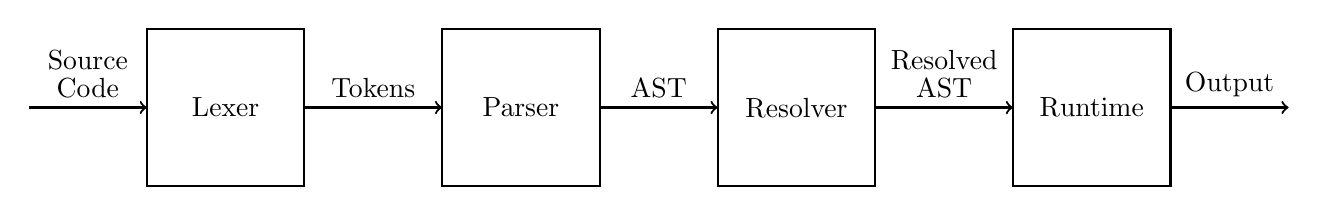
\begin{tikzpicture}
    % Draw the boxes
    \draw[thick] (-4.5, 0) rectangle (-2.5, 2);
    \draw[thick] (-0.75, 0) rectangle (1.25, 2);
    \draw[thick] (2.75, 0) rectangle (4.75, 2);
    \draw[thick] (6.50, 0) rectangle (8.50, 2);
    
    % Labels inside the boxes
    \node at (-3.5, 1) {Lexer};
    \node at (0.25, 1) {Parser};
    \node at (3.75, 1) {Resolver};
    \node at (7.5, 1) {Runtime};
    
    % Arrows and labels between boxes
    \draw[->, thick] (-2.5, 1) -- (-0.75, 1) node[midway, above] {Tokens};
    \draw[->, thick] (1.25, 1) -- (2.75, 1) node[midway, above] {AST};
    \draw[->, thick] (4.75, 1) -- (6.50, 1) node[midway, above] {\shortstack{Resolved \\ AST}};
    
    % Input and output arrows
    \draw[->, thick] (-6, 1) -- (-4.5, 1) node[midway, above] {\shortstack{Source \\ Code}};
    \draw[->, thick] (8.50, 1) -- (10, 1) node[midway, above] {Output};
  \end{tikzpicture}
  \caption{Box-Diagram representing the phases of the Bleach Interpreter.}
\end{figure}

\subsection{Lexer}
We recall that the goal of the lexer is to transform the received source code (which is viewed by it as a large string of characters) into a sequence of tokens that will be fed to the parser. Such transformation performed by the lexer is known as lexical analysis.

Regarding the possible tokens that can be generated during the lexical analysis, we list the types of tokens recognized by the lexer on Tables 4.2, 4.3 and 4.4:
\newpage
\begin{itemize}
    \item \textbf{Single-Character Tokens:}

    \begin{table}[h!]
        \centering
        \begin{minipage}{0.45\textwidth}
            \centering
            \begin{tabular}{|c|c|}
                \hline
                \textbf{Token Type} & \textbf{Token} \\
                \hline
                LEFT\_PAREN & \texttt{(} \\ \
                RIGHT\_PAREN & \texttt{)} \\ 
                LEFT\_BRACKET & \texttt{[} \\ 
                RIGHT\_BRACKET & \texttt{]} \\ 
                LEFT\_BRACE & \texttt{\{} \\ 
                RIGHT\_BRACE & \texttt{\}} \\ 
                COMMA & \texttt{,} \\ 
                DOT & \texttt{.} \\ \
                COLON & \texttt{:} \\ \
                SEMICOLON & \texttt{;} \\ 
                \hline
            \end{tabular}
            \caption{Single-Character Tokens - Pt. 1}
        \end{minipage}
        \hfill
        \begin{minipage}{0.45\textwidth}
            \centering
            \begin{tabular}{|c|c|}
                \hline
                \textbf{Token Type} & \textbf{Token} \\
                \hline
                QUESTION\_MARK & \texttt{?} \\ 
                PLUS & \texttt{+} \\ 
                MINUS & \texttt{-} \\ 
                STAR & \texttt{*} \\ 
                SLASH & \texttt{/} \\ 
                REMAINDER & \texttt{\%} \\ 
                BANG & \texttt{!} \\ 
                EQUAL & \texttt{=} \\ 
                GREATER & \texttt{>} \\ 
                LESS & \texttt{<} \\ 
                \hline
            \end{tabular}
            \caption{Single-Character Tokens - Pt. 2}
        \end{minipage}
    \end{table}

    \item \textbf{Double-Character Tokens:}
    \begin{table}[h!]
    \centering
        \begin{tabular}{|c|c|}
        \hline
        \textbf{Token Type} & \textbf{Token} \\ \hline
        ARROW & \texttt{->} \\
        EQUAL\_EQUAL & \texttt{==} \\
        EQUAL\_EQUAL & \texttt{!=} \\
        GREATER\_EQUAL & \texttt{>=} \\
        LESS\_EQUAL & \texttt{<=} \\ \hline     
        \end{tabular}
        \caption{Double-Character Tokens recognized by the lexer of Bleach's Interpreter.}
    \end{table}

    \item \textbf{Multi-Character Tokens:}
    \begin{table}[h!]
    \centering
        \begin{tabular}{|c|c|}
        \hline
        \textbf{Token Type} & \textbf{Token} \\ \hline
        IDENTIFIER & \texttt{(a-z|A-Z|\_)(a-z|A-Z|0-9|\_)\textsuperscript{*}} \\
        NUMBER & \texttt{[0-9]\textsuperscript{+}(.[0-9]\textsuperscript{+})?} \\
        STRING & \texttt{"(any ASCII character)\textsuperscript{*}"} \\ \hline      
        \end{tabular}
        \caption{Multi-Character Tokens recognized by the lexer of Bleach's Interpreter.}
    \end{table}

    \item \textbf{FILE\_END Token:} This token is a special one that the Bleach interpreter supports. It is responsible for signaling the end of a \texttt{.bch} file. This token has an empty string as its lexeme. Its addition will be discussed on section 4.5.
\end{itemize}

With respect to identifier tokens, it is important to provide the table of keywords of a programming language. In Bleach's case, this table is shown below:
\begin{table}[H]
    \centering
    \begin{tabular}{|c|c|c|}
    \hline
    \texttt{and} & \texttt{break} & \texttt{class}  \\ \hline
    \texttt{continue} & \texttt{do} & \texttt{elif}  \\ \hline
    \texttt{else} & \texttt{false} & \texttt{for}  \\ \hline
    \texttt{function} & \texttt{if} & \texttt{inherits} \\ \hline
    \texttt{lambda} & \texttt{let} & \texttt{method} \\ \hline
    \texttt{nil} & \texttt{or} & \texttt{print} \\ \hline
    \texttt{return} & \texttt{self} & \texttt{super} \\ \hline
    \texttt{true} & \texttt{while} &  \\ \hline
    \end{tabular}
    \caption{Table with all keywords available in Bleach.}
\end{table}

Regarding the implementation, the lexer was hand-written. It can successfully recognize string literals and number literals. It can also ignore whitespace characters, single-line comments and multi-line comments. On top of that, the lexer is able to successfully distinguish token that share the same initial characters on their lexemes by using the concept of lookahead and "maximal munch", both previously presented. The "maximal munch" concept is also used to identify tokens that have a keyword as their lexemes from tokens that have just an identifier as their lexemes. 

Lastly, the lexer is capable of identifying invalid characters, unterminated string literals, unterminated multi-line comments and misuse of the \texttt{':'} character.

\newpage

\subsection{Parser}
The goal of the parser is to transform the received sequence of tokens into an Abstract Syntax Tree (AST) that will be fed to the resolver of the interpreter. This conversion is known as syntax analysis.

Regarding the possible AST nodes to be generated during the syntax analysis, they can be divided into two groups of nodes (expressions and statements). These groups are structured as displayed in Table \ref{tab:ASTNodes}:

\begin{table}[h!]
\centering
    \begin{tabular}{|c|c|}
    \hline
    \textbf{Expr} & \textbf{Stmt} \\ \hline
    Assign & Block \\ \hline
    Binary & Break \\ \hline
    Call & Class \\ \hline
    Get & Continue \\ \hline
    Grouping & DoWhile \\ \hline
    LambdaFunction & Expression \\ \hline
    ListLiteral & For \\ \hline
    Literal & Function \\ \hline
    Logical & If \\ \hline
    Self & Print \\ \hline
    Set & Return \\ \hline
    Super & Var \\ \hline  
    Ternary & While \\ \hline
    Unary &  \\ \hline
    Variable &  \\ \hline
    \end{tabular}
    \caption{All possible types of AST nodes in the Bleach programming language. \newline}
    \label{tab:ASTNodes}  % Label for referencing the table
\end{table}


With respect to the parsing technique, the chosen one was the Recursive-Descent parsing technique. With this in mind, we present the BNF-grammar of Bleach in Figure 4.50: \newline

\begin{figure}
    \centering
\scalebox{0.70}{
\[
\begin{array}{rcl}
\texttt{program}   & ::= & \texttt{statement\textsuperscript{*} EOF} \\[1pt]
\texttt{statement} & ::= & \texttt{block | breakStmt | classDeclStmt | continueStmt | doWhileStmt} \\
                     &     & \texttt{| exprStmt | forStmt | funcDeclStmt | ifStmt | printStmt} \\
                     &     & \texttt{| returnStmt | varStmt | whileStmt} \\[1pt]
\texttt{block} & ::= & \texttt{"\{" statement\textsuperscript{*} "\}"} \\
\texttt{breakStmt} & ::= & \texttt{"break" ";"} \\[1pt]
\texttt{classDeclStmt} & ::= & \texttt{"class" IDENTIFIER ( "inherits" IDENTIFIER )? "\{" methodDeclStmt\textsuperscript{*} "\}"} \\[1pt]
\texttt{methodDeclStmt} & ::= & \texttt{"method" method} \\[1pt]
\texttt{method} & ::= & \texttt{IDENTIFIER "(" parameters? ")" block} \\[1pt]
\texttt{continueStmt} & ::= & \texttt{"continue" ";"} \\[1pt]
\texttt{doWhileStmt} & ::= & \texttt{"do" block "while" "(" expression ")" ";"} \\[1pt]
\texttt{exprStmt} & ::= & \texttt{expression ";"} \\[1pt]
\texttt{forStmt} & ::= & \texttt{"for" "(" ( varDecl | exprStmt | ";" ) expression? ";" expression? ")" block} \\[1pt]
\texttt{funcDeclStmt} & ::= & \texttt{"function" function} \\[1pt]
\texttt{function} & ::= & \texttt{IDENTIFIER "(" parameters? ")" block} \\[1pt]
\texttt{parameters} & ::= & \texttt{IDENTIFIER ( "," IDENTIFIER )\textsuperscript{*}} \\[1pt]
\texttt{ifStmt} & ::= & \texttt{"if" "(" expression ")" statement ("elif" "(" expression ")" statement )*} \\[1pt]
\texttt{} & & \texttt{( "else" statement )? } \\[1pt]
\texttt{printStmt} & ::= & \texttt{"print" expression ";"} \\[1pt]
\texttt{returnStmt} & ::= & \texttt{"return" expression? ";"} \\[1pt]
\texttt{varDeclStmt} & ::= & \texttt{"let" IDENTIFIER ("=" expression )? ";"} \\[1pt]
\texttt{whileStmt} & ::= & \texttt{"while" "(" expression ")" block} \\[1pt]
\texttt{expression} & ::= & \texttt{assignment} \\[1pt]
\texttt{assignment} & ::= & \texttt{( call "." )? IDENTIFIER "=" assignment | ternary} \\[1pt]
\texttt{ternary} & ::= & \texttt{logic\_or ( "?" expression ":" expression )*} \\[1pt]
\texttt{logic\_or} & ::= & \texttt{logic\_and ( "or" logic\_and )*} \\[1pt]
\texttt{logic\_and} & ::= & \texttt{equality ( "and" equality )*} \\[1pt]
\texttt{equality} & ::= & \texttt{comparison ( ( "==" | "!=" ) comparison )*} \\[1pt]
\texttt{comparison} & ::= & \texttt{term ( ( ">" | ">=" | "<" | "<=" ) term )*} \\[1pt]
\texttt{term} & ::= & \texttt{factor ( ( "+" | "-" ) factor )*} \\[1pt]
\texttt{factor} & ::= & \texttt{unary ( ( "*" | "/" | "\%" ) unary )*} \\[1pt]
\texttt{unary} & ::= & \texttt{( "!" | "-" ) unary | call} \\[1pt]
\texttt{call} & ::= & \texttt{primary ( "(" arguments? ")" | "." IDENTIFIER )*} \\[1pt]
\texttt{arguments} & ::= & \texttt{expression ( "," expression )*} \\[1pt]
\texttt{primary} & ::= & \texttt{"true" | "false" | "nil" | NUMBER | STRING | IDENTIFIER | "super" "." IDENTIFIER }  \\[1pt]
\texttt{} &  & \texttt{| "(" expression ")" | "[" ( expression ( "," expression )* )? "]"} \\[1pt]
\texttt{lambdaFunctionExpr} & ::= & \texttt{"lambda" "->"  "(" parameters? ")" block} \\[1pt]
\end{array}
\]
}
    \caption{BNF-Grammar of Bleach.}
    \label{fig:enter-label}
\end{figure}



\newpage

In other words, the grammar of Bleach is defined by the set of rules that have been just presented. Such rules are the entities that control how expressions and statements are formed in this particular programming language.

For example, by analyzing the BNF-Grammar presented, it becomes clear to the reader the precedence of the binary arithmetical operators. The operators \texttt{"*"}, \texttt{"/"} and \texttt{"\%"} have the same precedence among them, but have more precedence when compared to the operators \texttt{"+"} and \texttt{"-"}, which also have the same precedence among them.

As mentioned previously, the parser is implemented with a top-down approach called Recursive-Descent parsing. In the case of the implemented interpreter, this parser is hand-written, since, as explained in Chapter 2, this particular parsing technique is basically a direct translation of a grammar to code that makes use of recursive functions, which makes its implementation straight-forward.

Concerning the parsing phase and the AST generation, as explained in Chapter 2, a recursive-descent parser starts the parsing process from the outermost grammar rule, which in Bleach's case is the \texttt{program} rule, and executes the process already explained when it comes to a top-down recursive descent parsing strategy.

One of the most important aspects of parsing is error reporting. In the parsing phase, the kind of error that is reported is commonly know as syntax error.

Following the guidelines presented in Chapter 2, to deal with syntax errors, the parser component implements the ideas of "panic mode" and "error recovery". When the parser enters such mode, it needs to keep parsing process going until and continue to report more valid syntax errors until it reaches the end of the tokens sequence. To achieve this goal, the parser has a synchronization mechanism that looks for "synchronization points" from which the parser can continue the parsing process without issues. When in synchronization the parser ignores any tokens until it finds one that is a "synchronization point" and, in Bleach's case, such points are between statements.

\subsection{Resolver}
The resolver is a component of the interpreter responsible for performing a semantic analysis through the AST generated by the parser. To do such traversal on the AST, the Visitor design pattern is used, since it is better suited for this type of task, as previously explained. 

Even though the resolver performs a semantic analysis pass over the source code, it is a simple and straight-forward one. This pass is in charge of discovering where variables were declared and guaranteeing that they are properly used within their scope. This component is able to resolve variable references by traversing the AST generated by the parser and associating each variable with its corresponding environment/scope inside which it was defined.

As a way to make these associations correctly the resolver has a stack of scopes in which the the scope at the top of the stack is the current scope being analyzed. For instance, the resolver component always creates a new scope and pushes it to the top of the mentioned stack every time it starts the visiting of one of the following types of AST node: \texttt{LambdaFunction}, \texttt{Block}, \texttt{Class}, \texttt{DoWhile}, \texttt{For}, \texttt{While}. When the visiting of such nodes is ended, the scope at the top of the previously mentioned stack is popped and the AST traversal continues. Still on this aspect, the resolver is responsible for providing the runtime with the information necessary to find the correct variable to which a certain identifier is referring to in the chain of environments created at runtime.

The resolver is also able of reporting different types of errors related to variable declaration and usage.
\begin{itemize}
    \item The resolver is able to find a variable re-declaration inside the same scope and report it as an error.
    \item The resolver is also able to identify that a variable is being used in its own initializer expression and report it as an error.   
\end{itemize}

On top of that, the resolver component of the Bleach interpreter is capable of catching other errors, such as:
\begin{itemize}
    \item Usage of the \texttt{self} keyword outside of a class declaration statement.
    \item Usage of the \texttt{super} keyword outside of a class declaration statement.
    \item Usage of the \texttt{super} keyword inside a class declaration statement that is not a subclass from another class.
    \item Usage of the \texttt{break} keyword outside of any loop statement (\texttt{for}, \texttt{do-while}, \texttt{while}).
    \item Usage of the \texttt{continue} keyword outside of any loop statement (\texttt{for}, \texttt{do-while}, \texttt{while}).
    \item Usage of a class as the superclass of itself.
    \item Usage of the \texttt{return} keyword outside of a function, anonymous/lambda function or method.
    \item Usage of the \texttt{return} keyword inside the \texttt{init} method of a class declaration statement.
\end{itemize}

\subsection{Runtime}
The runtime is the last component of the interpreter. In short, this component is responsible for executing statements, evaluating expressions, performing control-flow, managing scopes with their variables and respective values and also throwing runtime errors whenever required. From a different point of view, the runtime can be viewed as the engine responsible for executing code accordingly with the semantics of the implemented programming language.

This type of interpreter works, as explained in Chapter 2, by executing a recursive traversal on the AST and performing different actions depending on the type of the AST's node that is currently being visited. All types of AST's node were also previously presented in Table \ref{tab:ASTNodes}.

Dealing with the first group of AST nodes, the ones that represent expressions, the behavior of the runtime will fundamentally be the same: it will visit the node that represents an expression, then evaluate the expression, finally it will produce the value from said expression and will move on to continue the recursive traversal of the abstract syntax tree. 
However, the evaluation of these AST expression nodes consistently varies accordingly with the specific expression in question. A rundown of these specific behaviors regarding each type of expression node is presented beneath:
\begin{itemize}
    \item \textbf{Assign:} When visiting this kind of expression node, the interpreter first evaluates the RHS (right-hand side) of this expression node. This evaluation will produce a value that must be assigned to the LHS (left-hand side) of this very same node. However, the evaluation of the LHS is different. This one evaluates to a location in-memory in which the value obtained through the evaluation of the RHS will be stored. In order to find out the correct memory location, the runtime makes use of information previously computed by the resolver about variable resolution and environments. By default, this visiting returns the value from the RHS evaluation.
    \item \textbf{Binary:} When visiting this type of expression node, the interpreter first evaluates its left operand and, then, the right one. Finally, it performs the operation depending on the type of operator that this node stores and returns the result of such operation.
    \item \textbf{Call:} When visiting this sort of expression node, the interpreter first evaluates the callee of this node in order to figure out if it is a valid one (a function, an anonymous/function, a native function, a method, a class, or a method from the \texttt{list} and \texttt{str} built-in types). Once this is done, the interpreter evaluates each of the expressions that represent the arguments of the call and store such values appropriately. Finally, it makes the call to the callee passing the evaluated arguments. This sort of expression node returns the same thing the function that has been called returns.
    \item \textbf{Get:} When visiting this kind of expression node, the interpreter first evaluates the expression representing the entity on which the property is trying to be accessed. If such expression evaluates to an instance of a class, a value of type \texttt{list} or a value of type \texttt{str}, then the interpreter tries to find the value associated to the property and, finally, returns it.
    \item \textbf{Grouping:} When visiting this type of expression node, the interpreter just evaluates and, ultimately, returns the produced value by the nested expression within this type of node, since a Grouping node essentially represents a pair of parentheses.
    \item \textbf{LambdaFunction:} When visiting this kind of expression node, the interpreter just creates a runtime representation of the anonymous/lambda function by using the visited expression itself along with the current environment/scope that is in, since it will serve as the closure of such anonymous function.
    \item \textbf{ListLiteral:} When visiting this sort of expression node, the interpreter creates the runtime representation of a list. Then it evaluates each expression present inside the ListLiteral expression and appends the result to the runtime portrayal of the mentioned list. In the end, it returns such list.
    \item \textbf{Literal:} When visiting this type of expression node, the interpreter just evaluates the value associated with the literal and returns it.
    \item \textbf{Logical:} This expression node is a basically a specialization of the "Binary" node because it can only perform the following operations: \texttt{and}, \texttt{or}. Still, it evaluates the left operand first and, according to the left value and the operator itself, tries to perform a short-circuiting. If that's not possible, it evaluates the right operand, produces the corresponding value by following the rules of Boolean Algebra and, finally, returns the produced value.
    \item \textbf{Self:} When visiting this kind of expression node, the interpreter uses it and the token that represents that particular \texttt{self} keyword to figure out at which environment the required variable is at (remember that the \texttt{self} is a name that references the current instance of a class, making it, in practice a variable). Once at such environment, the interpreter returns the instance bound to such name.
    \item \textbf{Set:} The visiting process of this expression node is very similar to that of the "Get" node. In this particular expression node, the interpreter first evaluates the expression representing the value that works as the RHS. Then, the interpreter evaluates the expression that represents the entity that contains the attribute that is about to receive the generated RHS value. If the evaluation of the expression that represents an entity results in a valid value (an instance of a class), then the interpreter searches for the attribute inside such value (which will result in a LHS value) in order to perform the binding between them. Finally, this visiting process returns the RHS value.
    \item \textbf{Super:} When visiting this sort of expression node, the interpreter first retrieves the superclass of the class whose "Super" node is being currently visited. Once this is finished, the interpreter then retrieves the instance of the class whose "Super" node is being visited. Finally, the interpreter searches and returns the superclass version of the method required in the "Super" expression node.    
    \item \textbf{Ternary:} When visiting this particular expression node, the interpreter first evaluates its first operand, known as condition. If the result produced by such evaluation is \texttt{true}, then the ternary operator evaluates and returns its second operand, the one between \texttt{"?"} and \texttt{":"}. Otherwise, this operator evaluates and returns its third operand, the one that appears after \texttt{":"}.
    \item \textbf{Unary:} When visiting this type of expression node, the interpreter first evaluates its unique operand, commonly known as right operand. After this, it performs the operation, given the operator, on the operand, produces and, at last, returns the corresponding value.
    \item \textbf{Variable:} When visiting this type of expression node, the interpreter uses the expression node itself, which represents a variable usage, combined with the variable's token to figure out at which environment the required variable is at. Then, the runtime accesses that environment, retrieves and returns the value associated to the required variable. 
\end{itemize}

The second group of AST nodes is the one that contains nodes representing different kinds of statement, which can be called statement nodes. However, before showing each one, it is important to recall the reader that statements do not produce values. Keeping this in mind, there exists the following types of statement nodes:
\begin{itemize}
    \item \textbf{Block:} When visiting this kind of statement node, the interpreter first stores the current environment (the implementation of the concept of lexical scope). Then, sets the current environment of the interpreter to another that has been created and whose enclosing one is the one that has been on use before the interpreter started the visit to this statement node. On this new environment current environment, the interpreter executes the statements present in the "Block" node one-by-one from top to bottom. After finishing this, it restore the environments to the initial configuration before starting the visit of this type of statement node.
    \item \textbf{Break:} When visiting this sort of statement node, the interpreter just throws an instance of a "Break" entity that will be caught by the runtime when visiting any loop statement node (\texttt{do-while}, \texttt{for}, \texttt{while}) and dealt with by it. This entity is responsible for simulating the behavior of loop interruption at runtime caused by the use of a \texttt{break} statement.
    
    \item \textbf{Class:} When visiting this type of statement node, the interpreter first checks whether the node has an expression that might evaluate to a superclass. If that's the case, such expression is properly evaluated and its result is stored for later use. After this, the interpreter creates a binding at the current environment it is in between the class name and the \texttt{nil} value. If the "Class" statement node indeed has a superclass associated to it, a nesting environment is created and a binding between the name \texttt{super} and the runtime representation of the superclass is generated. Then, for each method declared inside this statement node, its respective runtime representation is generated and stored inside the runtime representation of the class in a way that associates the name of the method and its respective runtime depiction. At last, the runtime portrayal of the class is populated with the needed information.
    
    \item \textbf{Continue:} When visiting this kind of statement node, the interpreter just throws an instance of a "Continue" entity that will be caught by the runtime when visiting any loop statement node (\texttt{do-while}, \texttt{for}, \texttt{while}) and dealt with by it. This entity is responsible for simulating the behavior of interrupting an iteration of a loop and going to the next iteration by the use of a \texttt{continue} statement.
    
    \item \textbf{DoWhile:} When visiting this sort of statement node, the interpreter first saves the previous environment it was in, so it can restore it, once it has finished the execution of the "DoWhile" statement. After this, the interpreter makes the current environment store a new environment whose enclosing environment is the one that has just been saved and starts executing the statements present inside the block of the "DoWhile" statement, always checking whether the condition of such statement still evaluates to \texttt{true} after the execution of all statements present inside its block. Once this condition evaluates to \texttt{false}, the interpreter interrupts the execution of this loop and restores the initial environment that was previously stored.
    
    \item \textbf{Expression:} When visiting this type of statement node, the interpreter simply evaluates the expression present inside it, which results in the generation of a value.
    
    \item \textbf{For:} When visiting this kind of statement node, the interpreter first saves the previous environment it was in, so it can restore it, once it has finished the execution of the "For" statement. After this, the interpreter makes the current environment store a new environment whose enclosing environment is the one that has just been saved. Then, the interpreter executes the initializer statement present inside the "For" statement. Once this is done, it evaluates the expression that represents the condition of the "For" statement at beginning of each iteration. If the evaluation results in a "truthy" value, then the statement(s) present inside the block of the "For" statement, including the last special statement, usually called "increment statement". This goes on until the expression that represents the condition evaluates to a "falsey" value. As soon as this happens, the visiting of this node is complete.
    
    \item \textbf{Function:} When visiting this sort of statement node, the interpreter just creates the runtime representation of the function and creates a binding between the name of the function and its corresponding runtime portrayal in the current environment the runtime is currently in.
    
    \item \textbf{If:} When visiting this type of statement node, the interpreter first evaluates the expression associated with the "If" branch within this type of node. In case the produced value is a "truthy" one, the statement(s) associated with this clause are executed and the interpreter finishes this node visiting. If that's not the case, then the interpreter will check for the possible presence of "Elif" branches in this node (which are stored in a sequential manner). If they are indeed present, the interpreter evaluates the expression associated with each one in order until it finds one expression that, when evaluated, produces a "truthy" value, when this happens, the statement(s) associated to such clause are executed and this visiting is also terminated. Finally, the interpreter checks for the presence of an "Else" clause. If it exists, then its statement(s) are executed and this node visiting ends. 
    
    \item \textbf{Print:} When visiting this kind of statement node, the interpreter first evaluates the expression that is stored inside it. After this, it outputs the produced value to the standard output (terminal).
    
    \item \textbf{Return:} When visiting this sort of statement node, the interpreter checks whether there is an expression present inside such statement. If there is, then this expression is evaluated and the produced value is wrapped inside an entity that is thrown and will be caught by the caller of the function, anonymous function, native function, method. If there is not such expression, then the \texttt{nil} value is wrapped and thrown instead.
    
    \item \textbf{Var:} When visiting this type of statement, the interpreter checks whether there is an initializer expression for the variable declaration statement. If there is, then such expression is evaluated and the generated value is stored. Otherwise, by default the value \texttt{nil} is stored. At last, the interpreter performs a binding inside the current environment it is in between the name of the variable present inside the node and the respective value that was previously saved.
    
    \item \textbf{While:} When visiting this kind of statement, the interpreter first saves the previous environment it was in, so it can restore it, once it has finished the execution of the "While" statement. After this, the interpreter makes the current environment store a new environment whose enclosing environment is the one that has just been saved. Then, the interpreter starts to properly execute the "While" statement by at each iteration checking whether the condition of such statement evaluates to \texttt{true} and then executing its block of statements if that is indeed the case. Once this condition does not hold anymore, the interpreter does not execute this block of statements.

\end{itemize}

\section{Challenges, Decisions and Trade-Offs}
This section is dedicated to report the challenges faced when designing Bleach and implementing its Tree-Walk Interpreter as well as the decisions made, the reasoning behind them and trade-offs that rose from such decisions.

For structuring purposes, this section is organized as a list of challenges. The first group of challenges is about language design while the second one is about interpreter implementation challenges.

\begin{itemize}
    \item \textbf{Language Design Challenges, Decisions and Trade-Offs:}
    \begin{itemize}
        \item \textbf{Concept of "Truthy" and "Falsey" values}: Since popular programming languages like Ruby, Python, JavaScript and TypeScript started adopting this idea that every value has an associated notion of truthiness or falseness, it felt right to also adopt this philosophy in order to make Bleach modern and flexible. The question that rose from this adoption was: Which values should be considered 'truthy' and which should be considered 'falsey'? For the sake of design's simplicity and easiness when it came down to Bleach's implementation, the road taken by Ruby was also followed: the values \texttt{false} and \texttt{nil} are considered "falsey", while every other one is considered "truthy".
        
        \item \textbf{Inserting the concept of \texttt{nil} in Bleach:} This is undoubtedly an idea that may raise questions, specially since the creator of the concept itself, Tony Hoare, regrets inventing it, calling it "a billion dollar mistake" \cite{hoare_billion_dollar_mistake}. However, since Bleach and its interpreter implementation are heavily inspired by the "Crafting Interpreters" book \cite{nystrom2021crafting}, it took the same road as the language presented in that book simply because in a dynamically-typed language, which is Bleach's case, trying to exclude the idea of \texttt{nil} is more annoying than just allowing it. Thus, due to simplicity, it was adopted.
        
        \item \textbf{Absence of a \texttt{char} type:} The reader might have questions about the absence of this built-in data type in Bleach. The answer is: simplicity and familiarity. By not adding a new data type to the language, its type system becomes smaller. Moreover, the \texttt{str} type is enough to represent a such a type, since values of the \texttt{char} type can be viewed as values of the \texttt{str} that have length equal to \texttt{1}. In addition, it is important to remember that Bleach is dynamically-typed, which means that types are determined at runtime. Therefore, having a smaller type system reduces the amount of checks the runtime system must perform. Ultimately, popular dynamically-typed languages such as Python, Ruby and JavaScript adopted this same approach, thus, following it seems reasonable since this is a familiar pattern for students that had already contact with the mentioned languages.
        
        \item \textbf{A unique type (\texttt{num}) to represent numbers:} This design decision was taken having in mind simpleness and ease of use. One could argue that having a single numerical type has several disadvantages, like loss of integer precision, reduced performance and floating-point arithmetic issues. Even though all of these claims are correct, it is very important to remember that precision and optimized performance are not the main goals of Bleach. The main goal of the language proposed in this document is simplicity and easiness. Therefore, having just the \texttt{num} type reinforces this philosophy since having this unique type enables: consistency, unified arithmetic operations and unneeded type coercion or conversion.
        
        \item \textbf{Permission to re-declare global variables:} This decision has both pros and cons but, in the end, the pros seem to have a bigger impact than the cons. The major con is the visible inconsistency between local and global variables, since the local ones cannot be re-declared while global ones can. However, it is worth remembering the reader that the interpreter implemented for this language has two operating modes (one that activates an interactive session, a REPL, and another that reads and executes the content present inside a \texttt{.bch} file). Usually, in a REPL, the user might have difficulties on keeping track of which variable have been already declared and which have not. Following this reasoning, in order to make the user experience better when using the REPL, global variable re-declaration has been allowed.
        
        \item \textbf{Adoption of single inheritance instead of multiple inheritance:} This design decision was mainly motivated by clarity, simplicity and maintainability. Bleach was designed to be an educational tool, thus, there is encouragement to make it beginner-friendly and more accessible for students. With this in mind, dealing with single inheritance is easier than with multiple inheritance. In this vein, it is valuable explaining to the reader that single inheritance makes the whole hierarchy of classes less complicated to understand. A class can only have one "parent" class, with the exception of the base class. This structure makes inheritance more predictable and avoids the complexities of multiple inheritance, such as the "Diamond Problem" \cite{wikipedia_the_diamond_problem}.
    \end{itemize}


    \item \textbf{Tree-Walk Interpreter Implementation Challenges, Decisions and Trade-Offs:}
    \begin{itemize}
    
        \item \textbf{Lexer Implementation:} When it came to the building of the Lexer component, different strategies could have been adopted. In particular, a hand-written Lexer was the preferred one. The rationale behind this decision is that, even though there are tools capable of automatically generate a lexer given a set of rules defined by regular expressions (such as: Flex \cite{Flex} \cite{wiki_Flex}, JFLex \cite{klein2010jflex}), implementing one from scratch is not a hard task. Basically, all the programmer needs to do is deal with basic string processing and conditional logic, knowledge that is expected from CS students that are taking their undergraduate Compilers course. Moreover, demanding the students to implement the lexer themselves might be better a better approach to put their theoretical knowledge to practice instead of asking them to use semi-transparent automated tool solutions like Flex or JFlex, that abstract the nitty-gritty details of a lexer implementation.

        \item \textbf{Parser Implementation:} Regarding the choice of which way to follow when implementing the parser component, the most important factor taken into account was accessibility, easiness and simplicity. With these reasons in sight, the parser was implemented as a Top-Down Recursive Descent Parser. According to Nystrom \cite{nystrom2021crafting}, this kind of parser is intuitive and easy to understand, since it works as direct translation of the programming language grammar rules into functions/methods, easy to implement given the reason presented before and also simple to debug. The combination of these aspects make it a good choice for educational purposes, which is Bleach's main goal. One could argument that there are other kinds of parsers that could be used, such as LL(0) parser, LL(K) parser, LR(0) parser, LR(1) parser, LALR parser, among others. However, none of these approaches has a focus on education and learning. Besides, Nystrom affirms in \cite{nystrom2021crafting} that, even though, Recursive-Descent parsers are simple, they should not be underestimated since they are widely used in several popular programming language implementations: GCC, V8 (A JavaScript Runtime present in the Chrome browser) and the Roslyn Compiler (A C\# compiler written in C\#). Last but not least, there are tools that allow the automatic creation of parsers thanks to the use of tools like: ANTLR \cite{ANTLR}, Bison \cite{Bison} or Yacc \cite{johnson1975yacc} \cite{Yacc}. However, the use of such instruments might abstract important theoretical concepts of parsing theory. Therefore, the avoidance of such methodology.
        
        \item \textbf{Interpreter or Compiler? Why specifically a Tree-Walk Interpreter?} The decision to implement an interpreter instead of a compiler for Bleach was again influenced by easiness, simplicity and duration of an undergraduate thesis. In order to properly implement Bleach as a compiler, one is required to have a solid understanding of topics, such as: Intermediate Representation (IR) generation, optimizations and also code generation. As seen in Chapter 2, these topics are very broad when it comes to the concepts that are part of them. For example, if the compiler way was taken, there would be a need to decide about which IRs to use and how to properly use them. There would also be a decision about which optimizations should be implemented and, lastly, which path would be taken in the code generation phase: A bytecode virtual machine approach or an architecture specific machine code one?

        By taking into consideration all of these aspects, the choice of implementing an interpreter for Bleach seemed more achievable in the time frame of an undergraduate thesis and also easier. Nevertheless, it is important to make clear that Bleach can definitely be extended and implemented in other ways, according to the needs, available time and knowledge of the reader.

        Given that the interpreter road was taken, the decision about which type of interpreter should be implemented was still open. To address this situation, a Tree-Walk Interpreter was chosen. The reasoning behind this selection was rather simple: easiness to understand the topics being presented from the students point of view and focus on the language design, instead of worrying about the complex mechanisms needed to transform the source code into machine-code or byte-code. The easiness aspect comes from the fact that a Tree-Walk Interpreter works by performing a traversal through the AST generated by the parser and executing certain actions depending on the type of AST node that is being visited, by the time CS students took their Compilers course they should have already taken their Algorithms and Data Structures course, which addresses Trees, and therefore this makes it easier to follow the way such kind of interpreter works. Lastly, by focusing on language design it is expected that the students can focus more on the language semantics (how it behaves and what it can express), which for a beginner in this field might be more rewarding in terms of learning.

        
    \end{itemize}
\end{itemize}


\section{How Bleach Can Be Used In a Classroom Environment}
First of all, it is important to understand the conditions imposed in a classroom environment. In this context, knowing the period of time allocated to an academic semester in Compilers courses is essential.

Given the fact that, normally, an academic semester spans through 10 to 16 weeks depending on the internal organization of the university, for the sake of simplicity, it will be assumed that the academic semester spans through 15 weeks.

Lastly, we present a proposal of how Compilers courses that opt to use Bleach could be structured, considering the assumed time frame as its disposal and the tree-walk interpreter approach:
\begin{itemize}
    \item \textbf{Weeks 1 - 2 (Introduction to Programming Languages and Interpreters):}
        \begin{itemize}
            \item Provides an overview of programming languages design and implementation, by making a comparison between compilers and interpreters.
            \item Offers a review from certain topics related to Theory of Computation, for instance: Regular Expressions, Finite Automata (DFA and NFA) and Context-Free Grammars (CFG).
            \item Introduction of the Bleach programming language to the students.
        \end{itemize}
    
    \item \textbf{Weeks 3 - 4 (Lexing):}
        \begin{itemize}
            \item Provides an explanation about what is the purpose behind a lexer and what exactly lexical analysis is, while exposing related concepts, like: lexemes and tokens. Takes a deep dive into how a lexer actually works, supplying the theoretical baggage needed to implement one later on.
            \item Proposes the implementation of a lexer for the Bleach programming language. 
        \end{itemize}

    \newpage
    
    \item \textbf{Weeks 5 - 6 (Parsing):} 
        \begin{itemize}
            \item Provides an explanation about what is the purpose behind a parser and what exactly syntax analysis is, while exposing related concepts, like: ASTs, Bottom-Up and Top-Down parsing. Later on, explains the most important types of parsing (Recursive-Descent, LL(k) and LR(k)), while focusing in the first one, since it is the simplest of them all, but also robust, fast and reliable.
            \item Provides a more in-depth explanation about CFGs, if the need arises.
        \end{itemize}
    
    \item \textbf{Weeks 7 - 8 (Tree-Walk Interpretation):}
        \begin{itemize}
            \item Provides an explanation about how a tree-walk interpreter works in practice. This can be done by reviewing the concepts of trees and their respective types of traversal. Explanation about how each node in a syntax tree represents a different construct of a programming language, focusing on Bleach.
            \item Introduction to the Visitor design pattern, which is very useful to deal with the traversal of syntax trees
            \item Proposition of an assignment that deals with the initial implementation of the Bleach tree-walk interpreter, by first dealing with literal values, unary operators and binary operators.
        \end{itemize}

    
    \item \textbf{Week 9 (Variables, Scopes and Environments):}
        \begin{itemize}
            \item Provides an explanation about variable declaration statements, initializer of a variable, scopes (a conceptual idea), blocks (its visual representation) and environments (its respective implementation). 
            \item Explains how to manage variables that are stored in different scopes and the concept of variable shadowing.
            \item Proposition of a practice assignment to extend Bleach, so it can support the taught concepts.
        \end{itemize}

    \item \textbf{Week 10 (Control Flow Structures):}
        \begin{itemize}
            \item Provides an explanation about how control flow structures work behind the scenes. Explanation of how implement the most basic of these structures (\texttt{if} statement and \texttt{while} loop).
            \item Proposition of a programming assignment to extend Bleach in order for it support such structures.
            \item Proposition of bonus challenges that make the students think about concepts that have not been directly taught but can be learned through different types of references, such as: Addition of support for \texttt{for} and \texttt{while} loops (as well as support for the \texttt{break} and \texttt{continue} statements) and also for \texttt{else if} and \texttt{else} clauses as a mean to make the \texttt{if} statement more robust.
        \end{itemize}

    \item \textbf{Week 11 (Functions):}
        \begin{itemize}
            \item Provides explanation about how function declaration statements and function calls work behind the scenes. As well as how closures work and how one can implement such concepts.
            \item Proposition of an assignment to extend Bleach to support function declaration statements, function calls and closures.
            \item Proposition of a bonus challenge where students need to implement anonymous (lambda) functions.
        \end{itemize}

    \item \textbf{Week 12 (Standard Library):}
        \begin{itemize}
            \item Provides an explanation about what are standard libraries and native functions of a programming language, by providing a few examples of those present in languages like C and Python.
            \item Proposition of an assignment where students are asked to implement simple native functions for Bleach, following Bleach's documentation or other ideas.
        \end{itemize}
    
    \item \textbf{Week 13 (Resolving):}
        \begin{itemize}
            \item Provides explanation about what is static analysis, its role and its importance in the development of a programming language implementation, focusing on dynamically-typed languages, like Bleach, where such analysis is simpler and compared to statically-typed languages.
            \item Provides explanation about the importance of name resolution and how it can lead to unexpected bugs in during the interpretation of the AST (i.e., the runtime).
            \item Proposition of an assignment where students must implement their own Resolver component (a very simple component in an interpreter, where name resolution occurs).
        \end{itemize}
    
    \item \textbf{Week 14 (Object-Oriented Features):}
        \begin{itemize}
            \item Provides explanation about the essential object-oriented features present in Bleach: classes, instances, attributes, methods, the \texttt{self} keyword and single inheritance.
            \item Proposition of an assignment where students must extend Bleach in, so it can support all of the presented concepts and features.
            \item Proposition of a challenge asking students to implement static methods for classes and multiple inheritance instead of single inheritance.
        \end{itemize}

    \item \textbf{Week 15 (Projects Presentation and Final Exam):}
        \begin{itemize}
            \item In the last week of the academic semester, the students must present their tree-walk interpreters, as well as the extra challenge assignment that they were able to solve.
            \item Finally, apply final assessments and conduct project discussions.
        \end{itemize}

\end{itemize}

Teaching a Bleach implementation that employs the idea of Tree-Walk Interpreters can provide several benefits to the students, such as:
\begin{itemize}
    \item \textbf{Simplicity:} Generally speaking, a tree-walk interpreter is much simpler to implement than a full-compiler (it does not deal with the IR generation, optimization and code generation phases). Also, it does no go to deep into type systems, which can have their own courses given their complexity and vastness. Therefore, this might be ideal for students who are having their first contact with the world of programming language design and implementation without overwhelming them with the low-level concepts and implementations mentioned above.
    
    \item \textbf{Fast Execution and Iteration:} By implementing a tree-walk interpreter, students are able to see immediate results of their own work, since an interpreter essentially executes code from the generated AST, as explained in Chapter 2, making the connection between language syntax and runtime behavior more evident, while also motivating students since they can see the results of their work early on the course.
    
    \item \textbf{Hands-On Experience:} This approach enable students to obtain hands-on experience implementing a full interpreter, giving them a concrete understanding of how language constructs like variables, expressions, statements, control flow structures, functions, OOP features and simple static analysis work in practice.
    
    \item \textbf{Flexibility for Future Modifications:} This approach also encourages the students to experiment with language features (once students they have grasped the core concepts of tree-walk interpreters implementation) by adding new features, including but not restricted to the ones suggested earlier, which allows for creativity and deeper learning.
    
    \item \textbf{Solid Foundation for Future Learning:} By going through this methodology, it is expected that the students will be prepared to deal with more complex topics, such as bytecode interpreters, type systems and compilers with a deeper understanding of language runtime.
\end{itemize}

\begin{comment}

Complexities of type systems. They are usually taught after compilers and are a complex topic. Usually, such courses require an introductory compilers course first as a pre-requisite. Examples:

\begin{itemize}
    \item https://home.ttic.edu/~dreyer/course/ (ttic? - 2006)
    \item https://www.doc.ic.ac.uk/~svb/TSfPL/ (Imperial College London)
    \item https://stanford-cs242.github.io/f18/lectures/02-1-type-systems.html (Stanford)
    \item https://homepages.dcc.ufmg.br/~camarao/type-systems.html (UFMG)
    \item https://www.classes.cs.uchicago.edu/archive/2003/winter/33600-1/ (University of Chicago)
    \item https://www.mccormick.northwestern.edu/computer-science/academics/courses/descriptions/396-496-8.html (Northwestern University)
    \item http://lampwww.epfl.ch/teaching/archive/type\_systems/2004/ (EPFL)
\end{itemize}

\end{comment}

